
\documentclass[12pt,a4paper]{article}

\usepackage[T1]{fontenc}
\usepackage[utf8]{inputenc}
\usepackage[english]{babel}
\usepackage[margin=1in]{geometry}
\usepackage{graphicx}
\usepackage{setspace}
\usepackage{times}
\usepackage{titlesec}
\usepackage{amsmath, amssymb, amsthm, bm}
\usepackage{booktabs}
\usepackage{array}
\usepackage{caption}
\usepackage{subcaption}
\usepackage{float}
\usepackage{enumitem}
\usepackage{fancyhdr}
\usepackage{indentfirst}
\usepackage{xcolor}
\usepackage{listings}
\usepackage{algorithm}
\usepackage{algpseudocode}
\usepackage{csquotes}
\usepackage[round,authoryear]{natbib}
\setcitestyle{aysep={,}}
\setlength{\bibhang}{0.5in}
\usepackage{hyperref}

\hypersetup{
    colorlinks=true,
    linkcolor=black,
    citecolor=black,
    urlcolor=blue
}

\onehalfspacing
\setlength{\parindent}{0.5in}
\setlength{\parskip}{0pt}
\emergencystretch=2em

\titleformat{\section}
    {\normalfont\bfseries\large}{\thesection.}{0.5em}{}
\titleformat{\subsection}
    {\normalfont\bfseries}{\thesubsection.}{0.5em}{}

\pagestyle{fancy}
\fancyhf{}
\fancyhead[L]{AI-Powered Skill-Based Gig Matching for GigLink}
\fancyhead[R]{\thepage}
\renewcommand{\headrulewidth}{0.4pt}
\setlength{\headheight}{15pt}

\graphicspath{{../figures/}{figures/}}
\numberwithin{equation}{section}

\theoremstyle{definition}
\newtheorem{definition}{Definition}[section]
\newtheorem{assumption}{Assumption}
\theoremstyle{plain}
\newtheorem{theorem}{Theorem}[section]

\lstdefinestyle{py}{
  language=Python, basicstyle=\ttfamily\footnotesize\singlespacing, keywordstyle=\color{blue!60!black}\bfseries,
  commentstyle=\color{green!40!black}\itshape, stringstyle=\color{orange!70!black},
  numbers=left, numberstyle=\tiny\color{gray}, frame=single, rulecolor=\color{gray!50},
  breaklines=true, showstringspaces=false, columns=fullflexible, xleftmargin=1.5em, framexleftmargin=1.5em
}
\lstset{style=py}

\newcommand{\R}{\mathbb{R}}
\newcommand{\rel}{\mathrm{rel}}
% Generated by giglink_ai/make_tables.py from results/run_metadata.json
\newcommand{\DataGigsRaw}{52,977}
\newcommand{\DataGigsMapped}{42,029}
\newcommand{\DataMappedCats}{94}
\newcommand{\DataSeekers}{2,483}
\newcommand{\DataVocab}{2,814}
\newcommand{\DataGigTags}{5}
\newcommand{\DataSeekerTags}{24}
\newcommand{\DataResumeWords}{757}
\newcommand{\DataRelTwo}{109}
\newcommand{\DataRelTwoPct}{4.4\%}
\newcommand{\DataRuntimeMin}{17}
\DeclareMathOperator*{\argmax}{arg\,max}

\newcommand{\UniversityName}{Bulacan State University}
\newcommand{\CollegeName}{College of Science}
\newcommand{\CourseCode}{MCS 306 \& TWM 301}
\newcommand{\CourseDescription}{Introduction to Artificial Intelligence \& Technical Writing in Mathematics}
\newcommand{\AcademicYear}{Academic Year 2026--2027, First Semester}
\newcommand{\StudyTitle}{Skill-Based Gig Matching for GigLink Using TF-IDF, Latent Semantic Analysis, and Optimal Assignment}
\newcommand{\AuthorNames}{Kristiana T. Evangelista, Thealyne G. Jacinto, Jammele E. Perez,\\ Tifany B. Santos, and Justine S. Segubiense}
\newcommand{\CourseYearSection}{BSM CS 3B -- G2}
\newcommand{\InstructorName}{[Aarhus M. Dela Cruz, MCS 306]\\[2pt] [Aarhus M. Dela Cruz, TWM 301]}
\newcommand{\SubmissionDate}{October 31, 2026}


\newcommand{\BulSULogo}{assets/bulsu.png}
\newcommand{\COSLogo}{assets/college_of_science.png}


\newcommand{\LogoOrPlaceholder}[2]{%
  \IfFileExists{#1}%
    {\includegraphics[width=0.95\linewidth]{#1}}%
    {\fbox{\parbox[c][0.8\linewidth][c]{0.85\linewidth}{\centering\footnotesize #2\\logo}}}}

\begin{document}

\begin{titlepage}
    \centering

    \vspace*{0.3in}

    \begin{minipage}{0.22\textwidth}
        \centering
        \LogoOrPlaceholder{\BulSULogo}{BulSU}
    \end{minipage}
    \hfill
    \begin{minipage}{0.50\textwidth}
        \centering
        {\Large\bfseries \UniversityName\par}
        \vspace{0.15cm}
        {\large\bfseries \CollegeName\par}
        \vspace{0.15cm}
        {\normalsize \CourseCode: \CourseDescription\par}
        \vspace{0.15cm}
        {\normalsize \AcademicYear\par}
    \end{minipage}
    \hfill
    \begin{minipage}{0.22\textwidth}
        \centering
        \LogoOrPlaceholder{\COSLogo}{College of Science}
    \end{minipage}

    \vspace{0.9in}

    {\Large\bfseries MINI RESEARCH AND EXPOSITION PAPER\par}

    \vspace{0.45in}

    {\LARGE\bfseries \StudyTitle\par}

    \vspace{0.7in}

    {\large\bfseries Authors\par}
    \vspace{0.2cm}
    {\large \AuthorNames\par}

    \vspace{0.4in}

    {\large \CourseYearSection\par}

    \vfill

    {\normalsize Submitted to:\par}
    \vspace{0.15cm}
    {\normalsize\bfseries \ Aarhus M. Dela Cruz \par}

    \vspace{0.3in}

    {\normalsize \SubmissionDate\par}
\end{titlepage}

\pagenumbering{roman}
\setcounter{page}{1}

\begin{abstract}
\noindent GigLink is a proposed web-based marketplace in which students and young professionals of Bulacan State University take on short, task-based gigs posted by clients. One of its planned modules is \emph{provider matching}: given a gig posting, recommend the seekers who are most likely to have the required skills. This paper formulates provider matching as a content-based ranking problem followed by a one-to-one assignment problem. Gig descriptions and seeker profiles are represented as TF-IDF vectors in a vector space model; latent semantic analysis (LSA), computed with a randomized truncated singular value decomposition, maps them into a lower-dimensional concept space. A hybrid score combines LSA cosine similarity with the Jaccard similarity of skill tags, and when many gigs are open at the same time the linear assignment problem is solved exactly with a Hungarian-type algorithm. Because GigLink has not yet been deployed, the method is evaluated on real public data instead of synthetic data: 42,029 Upwork job posts serve as gigs and 2,483 LiveCareer resumes serve as seeker profiles, with relevance judged by a hand-written table that links each Upwork job category to the resume categories that do that work. Over 20 random samples of 400 gigs, the tuned hybrid model reached a test nDCG@10 of 0.438 (95\% CI $\pm$0.011) and a precision at 5 of 0.389, compared with 0.406 for LSA alone, 0.362 for TF-IDF, 0.324 for tag matching and 0.068 for random ranking; it beat every baseline on all 20 samples. Accuracy differed strongly between kinds of work, from about 0.75 for design and marketing gigs to below 0.2 for data-analytics and support gigs. Exact assignment collected 0.9\% (many seekers) to 6.1\% (few seekers) more relevance than greedy assignment, never double-booked a seeker, and ran faster. The study shows that simple, explainable linear-algebra methods work on real job and resume texts and are a feasible first AI component for GigLink, while also showing clearly where they are weak.
\end{abstract}

\noindent\textbf{Keywords:} recommender systems, vector space model, TF-IDF, latent semantic analysis, singular value decomposition, linear assignment problem, gig economy, job matching

\newpage
\tableofcontents
\newpage
\listoffigures
\listoftables
\newpage

\pagenumbering{arabic}
\setcounter{page}{1}

% ---------------------------------------------------------------------
\section{Introduction}\label{sec:intro}

\subsection{Background}
Many university students work while studying, both to cover living and school costs and to gain experience. In the Philippine setting, students commonly look for short-term work through referrals, social-media groups and messaging apps, which makes finding the right worker slow and unreliable for clients. GigLink is a proposed platform where clients post short, task-based gigs (for example tutoring, graphic design, writing, programming, photography, social media management, online selling and administrative support) and student seekers apply for them. A central need of such a platform is an intelligent matching mechanism that helps clients identify suitable seekers based on the skills and requirements specified in a gig posting. This study develops and evaluates that AI-based matching component.

Studies of online labour platforms show that clients rely heavily on profile information such as skills, ratings and rates when they choose freelancers \citep{ren2023hiring}, and recruitment recommender systems are an active research area \citep{freire2021erecruitment,deruijt2021job}. Industrial systems use learned embeddings to match jobs and candidates at large scale \citep{zhao2021embedding}. A small student platform such as GigLink, however, starts without click logs or hiring histories, so methods that need large amounts of interaction data are not yet usable. Matching people to tasks is a standard application of AI techniques for representing and retrieving information \citep{russell2021aima,manning2008introduction}. Content-based recommendation, which compares the \emph{content} of items and user profiles \citep{lops2011content}, does not need such history and is therefore a natural starting point.

\subsection{Problem statement}
When a client posts a gig, GigLink must rank hundreds of seeker profiles. Two practical difficulties make this harder than exact keyword search:
\begin{enumerate}[nosep]
  \item \textbf{Vocabulary mismatch.} A client may write \enquote{pubmat for our org event} while a seeker writes \enquote{poster and layout design}; both describe the same skill.
  \item \textbf{Different people describe themselves differently.} Real profiles vary widely in length, wording and how many skills they list, and clients describe the same kind of work in different ways. A matching method must work with this variety instead of assuming every user behaves the same.
\end{enumerate}
In addition, when many gigs are posted at once the platform should not send the same top seeker to every client, and in the full platform a seeker who is unavailable or too expensive for a gig should not be recommended.

\subsection{Objectives and research questions}
The general objective is to design, implement and evaluate a mathematically grounded AI matching method for GigLink. Specifically, we aim to answer:
\begin{description}[nosep,font=\normalfont\bfseries]
  \item[RQ1] How accurately do text-based (TF-IDF, LSA), tag-based (Jaccard) and hybrid models rank seekers, compared with random and keyword baselines?
  \item[RQ2] How robust are these models when seeker profiles are shorter or list fewer skills?
  \item[RQ3] Does solving a global assignment problem give better simultaneous matches than greedy or independent recommendations?
  \item[RQ4] What numerical settings (SVD rank and iteration count) and computational costs does the method require?
\end{description}

\subsection{Why this model}
We compared four candidate AI features for GigLink: a chatbot assistant, intelligent search, collaborative filtering and content-based skill matching. Collaborative filtering needs interaction history that does not exist yet, and a chatbot is difficult to evaluate quantitatively within the time available. Content-based matching works from the first day, rests on well-understood linear algebra (vectors, inner products, the singular value decomposition) and combinatorial optimisation (the assignment problem), is explainable to users (\enquote{matched because of: logo design, poster design}), and directly implements a planned GigLink module. It therefore offers the best balance of feasibility, mathematical depth and research value for this project.

\subsection{Scope and data statement}
GigLink is not yet deployed, so it has no user data of its own. Instead of generating artificial data, we evaluate the method on two \textbf{real, publicly available datasets} (Section~\ref{sec:data}): job posts that clients wrote on the freelancing platform Upwork, which play the role of GigLink gigs, and resumes that real job seekers wrote on the LiveCareer website, which play the role of GigLink seeker profiles. \textbf{No synthetic data are used anywhere in this study.} Because no public dataset records who was actually hired for which post, relevance is judged with an explicit category-compatibility table (Section~\ref{sec:data}). The results therefore measure how well the methods match real job texts to real resumes of the right field; they are \emph{not} measurements of GigLink users. Table~\ref{tab:status} at the end of Section~\ref{sec:discussion} lists which parts are implemented and tested and which are only proposed.

% ---------------------------------------------------------------------
\section{Preliminaries}\label{sec:prelim}

Throughout, vectors are columns, $\|\bm{x}\|_2$ is the Euclidean norm and $|A|$ is the size of a finite set $A$. There are $m$ gigs indexed by $g$ and $n$ seekers indexed by $s$.

\subsection{Vector space model and TF-IDF}
In the vector space model \citep{salton1975vector}, each document $d$ (a gig description or a seeker bio) becomes a vector in $\R^{|V|}$, where $V$ is the vocabulary of distinct words after removing common English stop-words.

\begin{definition}[TF-IDF weight]
Let $\mathrm{tf}_{t,d}$ be the number of times term $t$ occurs in document $d$, $N$ the number of documents and $\mathrm{df}_t$ the number of documents containing $t$. With sublinear term frequency and smoothed inverse document frequency \citep{salton1988term,manning2008introduction},
\begin{equation}
  w_{t,d} = \bigl(1+\ln \mathrm{tf}_{t,d}\bigr)\cdot\Bigl(1+\ln\frac{1+N}{1+\mathrm{df}_t}\Bigr) \quad (\mathrm{tf}_{t,d}>0), \qquad w_{t,d}=0 \text{ otherwise.}
  \label{eq:tfidf}
\end{equation}
The document vector is normalised, $\bm{x}_d = \bm{w}_d/\|\bm{w}_d\|_2$.
\end{definition}
The idf factor gives rare, informative words (\enquote{calculus}) more weight than words that appear everywhere (\enquote{student}).

\begin{definition}[Cosine similarity]
For non-zero $\bm{u},\bm{v}\in\R^p$, $\cos(\bm{u},\bm{v}) = \dfrac{\bm{u}^\top\bm{v}}{\|\bm{u}\|_2\|\bm{v}\|_2}$. For unit vectors this is simply the inner product $\bm{u}^\top\bm{v}$, and for non-negative TF-IDF vectors it lies in $[0,1]$.
\label{def:cos}
\end{definition}

\subsection{Singular value decomposition and latent semantic analysis}
Stack the $N$ unit document vectors as rows of $X\in\R^{N\times|V|}$.

\begin{theorem}[SVD and best low-rank approximation]
Every real matrix has a factorisation $X = U\Sigma V^\top$ with $U, V$ orthogonal and $\Sigma$ diagonal with $\sigma_1\ge\sigma_2\ge\dots\ge 0$. For $k<\operatorname{rank}(X)$, the truncation $X_k = U_k\Sigma_kV_k^\top$ that keeps the $k$ largest singular values minimises $\|X-Y\|_F$ over all matrices $Y$ of rank at most $k$, with $\|X-X_k\|_F^2=\sum_{i>k}\sigma_i^2$ \citep{eckart1936approximation}.
\end{theorem}

Latent semantic analysis \citep{deerwester1990lsa} represents document $d$ by the $k$-dimensional vector
\begin{equation}
  \bm{z}_d = V_k^\top\bm{x}_d \in\R^k \quad(\text{equivalently the $d$-th row of } U_k\Sigma_k), \qquad \hat{\bm{z}}_d = \bm{z}_d/\|\bm{z}_d\|_2 .
  \label{eq:lsa}
\end{equation}
Words that tend to appear in similar documents load on the same singular vectors, so two documents can be close in the latent space even when they share few exact words. This is the property we hope will reduce vocabulary mismatch.

\paragraph{Randomized truncated SVD.} Computing only the top $k$ singular triplets is done with the randomized range finder of \citet{halko2011finding}: draw a Gaussian test matrix $\Omega\in\R^{|V|\times(k+p)}$ (oversampling $p$), form $Y=(XX^\top)^qX\Omega$ with $q$ \emph{power iterations}, orthonormalise $Y=QR$, and take the exact SVD of the small matrix $B=Q^\top X$. Power iterations sharpen the decay of the spectrum: in the error bound of \citet{halko2011finding}, the constant multiplying $\sigma_{k+1}$ is raised to the power $1/(2q+1)$, so the error approaches the optimal value $\sigma_{k+1}$ as $q$ grows. The number of power iterations $q$ is the main iteration parameter of our method, and Section~\ref{sec:svdconv} measures its effect.

\subsection{Set similarity}
\begin{definition}[Jaccard similarity]
For finite sets $A,B$, $J(A,B)=|A\cap B|/|A\cup B|$, with $J(\emptyset,\emptyset)=0$. If $\bm{a},\bm{b}\in\{0,1\}^{|\mathcal{K}|}$ are the indicator vectors of $A,B$ over a skill list $\mathcal{K}$, then $|A\cap B|=\bm{a}^\top\bm{b}$ and $|A\cup B| = \bm{a}^\top\bm{1}+\bm{b}^\top\bm{1}-\bm{a}^\top\bm{b}$, which lets all gig--seeker pairs be computed with one matrix product.
\end{definition}

\subsection{The linear assignment problem}
Given a utility matrix $H\in\R^{m\times n}$, the (rectangular) linear assignment problem is
\begin{equation}
\begin{aligned}
  \max_{x}\; & \sum_{g=1}^{m}\sum_{s=1}^{n} H_{gs}\,x_{gs}\\
  \text{s.t. }& \textstyle\sum_{s} x_{gs}\le 1 \;\;\forall g, \qquad \sum_{g} x_{gs}\le 1\;\;\forall s, \qquad x_{gs}\in\{0,1\}.
\end{aligned}
\label{eq:lap}
\end{equation}
Its constraint matrix is totally unimodular, so the linear-programming relaxation already has an integral optimum, and the problem can be solved exactly in polynomial time by the Hungarian method \citep{kuhn1955hungarian}. SciPy's \texttt{linear\_sum\_assignment} implements a shortest augmenting path variant described by \citet{crouse2016implementing}, with worst-case time $O(n^3)$ for square problems.

\subsection{Ranking evaluation metrics}
For gig $g$, let $\pi_g(i)$ be the seeker placed at rank $i$ and $\rel_{g,s}\in\{0,1,2\}$ the graded ground-truth relevance; a seeker is \emph{relevant} when $\rel= 2$. Let $\mathcal{R}_g$ be the set of relevant seekers for $g$. Then
\begin{align}
  \mathrm{P@}k &= \frac{1}{k}\sum_{i=1}^{k}\mathbf{1}[\rel_{g,\pi_g(i)}\ge 2], \qquad
  \mathrm{R@}k = \frac{1}{|\mathcal{R}_g|}\sum_{i=1}^{k}\mathbf{1}[\rel_{g,\pi_g(i)}\ge 2], \label{eq:pr}\\
  \mathrm{DCG@}k &= \sum_{i=1}^{k}\frac{2^{\rel_{g,\pi_g(i)}}-1}{\log_2(i+1)}, \qquad
  \mathrm{nDCG@}k = \frac{\mathrm{DCG@}k}{\mathrm{IDCG@}k}, \label{eq:ndcg}\\
  \mathrm{RR} &= 1/\min\{i:\rel_{g,\pi_g(i)}\ge 2\}, \label{eq:mrr}
\end{align}
where IDCG@$k$ is the DCG of the ideal ordering \citep{jarvelin2002cumulated}. Each metric is averaged over gigs (MRR is the mean of RR). All four lie in $[0,1]$ and larger is better. nDCG@10 is our primary metric because it rewards putting the \emph{most} suitable seekers first and handles graded relevance.

% ---------------------------------------------------------------------
\section{Methods and Applications}\label{sec:methods}

\subsection{Model description}\label{sec:model}

\paragraph{Inputs.} For each gig $g$: the free-text title and description written by the client, and the set of required skill tags $T_g$ that the client selected on Upwork (for example \emph{logo design}, \emph{adobe illustrator}). For each seeker $s$: the free text of the resume, and a set of skill tags $\tilde T_s$. Resumes do not come with tags, so $\tilde T_s$ is the set of Upwork skill phrases (from the shared skill list $\mathcal{K}$, Section~\ref{sec:data}) that occur word-for-word in the resume.

\paragraph{Similarity components.} Text similarity $c_{gs}=\hat{\bm z}_g^\top\hat{\bm z}_s$ (LSA, Eq.~\ref{eq:lsa}) or $c_{gs}=\bm{x}_g^\top\bm{x}_s$ (TF-IDF, Eq.~\ref{eq:tfidf}), and tag similarity $j_{gs}=J(T_g,\tilde T_s)$.

\paragraph{Hybrid score.} With a weight $\alpha\in[0,1]$,
\begin{equation}
  H_{gs} = \alpha\,c_{gs} + (1-\alpha)\,j_{gs}.
  \label{eq:hybrid}
\end{equation}
This is a convex combination of two similarities in $[0,1]$: $\alpha=1$ uses text only and $\alpha=0$ uses tags only. For each gig the seekers are ranked by decreasing $H_{gs}$.

\paragraph{Feasibility constraints (platform design).} In the GigLink application a pair should only be recommended when the seeker's schedule overlaps the gig's working days and the expected cost fits the budget,
\begin{equation}
  F_{gs} = \mathbf{1}\bigl[D_g\cap D_s\neq\emptyset\bigr]\cdot\mathbf{1}\bigl[\rho_s h_g\le b_g\bigr],
  \label{eq:feas}
\end{equation}
with infeasible pairs moved to the bottom of the ranking ($H_{gs}\gets-\infty$). The code supports this filter, but the public resumes contain neither availability nor hourly rates, so \textbf{the constraint could not be evaluated on real data} and every pair is treated as feasible in the experiments ($F\equiv 1$).

\paragraph{Assignment.} When all $m$ gigs are matched at once, we solve Problem~\eqref{eq:lap} with $H$ from Eq.~\eqref{eq:hybrid}. Infeasible pairs, when known, are forbidden by giving them utility $-10^6$ (any forbidden pair the solver still returns, which only happens when a gig has no feasible seeker left, is discarded).

\paragraph{Assumptions.}
\begin{assumption}\label{as:text} Job posts and resumes mention the skills involved, possibly in different words; there is no deliberate deception.\end{assumption}
\begin{assumption}\label{as:gt} A resume is suitable for a gig when the person works in the field that the gig belongs to, as recorded by the category-compatibility table; work quality, price and availability are \emph{not} part of the ground truth (see Section~\ref{sec:limits}).\end{assumption}
\begin{assumption}\label{as:one} In the assignment experiment each gig needs one seeker and each seeker takes at most one gig in the matching round.\end{assumption}

\subsection{Dataset}\label{sec:data}
\paragraph{Why these datasets.} Our instructor required real rather than synthetic data, and GigLink itself has no users yet. We therefore chose two public Kaggle datasets that mirror the two sides of the GigLink marketplace. Both were written by real people for real job searches, both are in English, and their records are reproduced unchanged in our pipeline; only parsing and lower-casing are applied.

\paragraph{Gigs: Upwork job posts \citep{upworkdata}.} \DataGigsRaw{} job posts collected from Upwork's public job feed between December 2023 and February 2024. Each post has a title, a description, the pay type (hourly or fixed price) with its rate or budget, the client's country, and, embedded in the description text, the Upwork \emph{category} chosen by the client (220 different categories, e.g.\ \emph{Graphic Design}, \emph{Data Entry}, \emph{Video Editing}) and the Upwork \emph{skill tags} the client attached (median \DataGigTags{} tags per post). Upwork is the largest general freelancing platform, and its short, task-based posts are the closest public analogue to GigLink gigs.

\paragraph{Seekers: LiveCareer resumes \citep{resumedata}.} \DataSeekers{} resumes of real job seekers collected from the LiveCareer website, each filed under one of 24 job categories (e.g.\ \textsc{designer}, \textsc{accountant}, \textsc{information-technology}, \textsc{chef}). Names, companies and contact details are replaced by placeholders in the source, so no personal information is processed. A resume has a median of \DataResumeWords{} words. The resumes are much longer and more varied than the job posts, and some categories (chef, aviation, agriculture, healthcare) have no matching Upwork work at all, so they act as realistic distractors.

\paragraph{Skill tags for resumes.} The shared skill list $\mathcal{K}$ contains the \DataVocab{} Upwork skill tags of at most four words that occur in at least five job posts. A resume receives a tag when the tag phrase occurs in it as a whole sequence of words (\texttt{extract\_tags} in \texttt{real\_data.py}); the median resume receives \DataSeekerTags{} tags. Some of these tags are generic words such as \emph{business} or \emph{marketing}, which is part of the real difficulty of the task.

\paragraph{Ground truth.} No public dataset records who was hired for which Upwork post, so we judge relevance with a \textbf{category-compatibility table} (\texttt{data/category\_map.csv}) that we wrote by hand before running any model. For each of the \DataMappedCats{} most common Upwork categories it names the resume category that does that work (\emph{primary}) and up to three categories that do closely related work (\emph{related}); for example \emph{Logo Design} $\to$ \textsc{designer} (primary), \textsc{arts} and \textsc{digital-media} (related). Graded relevance is
\begin{equation}
\rel_{gs} = \begin{cases}2 & \text{the resume's category is the primary category for gig } g,\\ 1 & \text{it is a related category},\\ 0 & \text{otherwise.}\end{cases}
\label{eq:gt}
\end{equation}
The table uses only the two category labels, which no model sees, so the models are graded against an outside judgement rather than against their own inputs. Upwork posts in categories with no clear resume counterpart (for example \emph{General Virtual Assistance} or \emph{Creative Writing}) are left out, which keeps \DataGigsMapped{} of the job posts. In a typical sample, \DataRelTwo{} resumes are relevant ($\rel=2$) to each gig, about \DataRelTwoPct{} of all resumes.

\paragraph{Sampling.} For each random sample $R$ we draw 400 gigs without replacement from the mapped job posts and rank all \DataSeekers{} resumes for each of them. Different samples contain different gigs, so the spread over samples shows how much the results depend on which posts happen to be chosen.

\subsection{Experimental procedure}
\begin{enumerate}[nosep]
  \item For each random sample $R=0,\dots,19$, draw 400 gigs and split them at random into 200 \emph{validation} and 200 \emph{test} gigs; the seeker pool is always all resumes.
  \item Compute all score matrices (Random, Keyword, Jaccard, TF-IDF, LSA). \emph{Keyword} counts distinct shared words without weighting; \emph{Random} draws uniform scores.
  \item Tune the hybrid model by grid search on the validation gigs only: text source $\in\{\text{TF-IDF},\text{LSA}\}$ and $\alpha\in\{0,0.1,\dots,1\}$ (22 combinations), maximising nDCG@10.
  \item Evaluate every method on the test gigs, which were never used for tuning.
  \item Run ablations, robustness sweeps (5 samples per level), the assignment experiment (all 400 sampled gigs), an SVD convergence study and a runtime study.
  \item Report mean, standard deviation and a $t$-based 95\% confidence interval over samples, and compare the hybrid with each baseline by a paired $t$-test and a Wilcoxon signed-rank test \citep{wilcoxon1945individual} on the same samples.
\end{enumerate}

\subsection{Implementation and code}\label{sec:impl}
The implementation is in Python~3 with NumPy \citep{harris2020numpy}, SciPy \citep{virtanen2020scipy}, scikit-learn \citep{pedregosa2011scikit}, pandas and Matplotlib \citep{hunter2007matplotlib}. The full code, with comments, unit tests and instructions, is in the project's Git repository (\texttt{giglink\_ai/}). Table~\ref{tab:params} lists every numerical setting.

\begin{table}[htbp]
\centering\footnotesize
\caption{Numerical settings used in all experiments.}\label{tab:params}
\resizebox{\linewidth}{!}{%
\begin{tabular}{lll}
\toprule
Parameter & Value & Where set \\
\midrule
Gigs per sample / seekers & 400 / all \DataSeekers{} resumes & \texttt{RealConfig} \\
Random samples (main / sweeps) & 20 / 5 & \texttt{experiments.py} \\
Skill list $\mathcal{K}$ & tags used by $\ge 5$ posts, $\le 4$ words & \texttt{skill\_vocabulary} \\
LSA rank $k$ & 40 & \texttt{LSA\_K} \\
Power iterations $q$ (randomized SVD) & 7 & \texttt{SVD\_ITERS} \\
Oversampling $p$ & 10 (scikit-learn default) & \texttt{TruncatedSVD} \\
Exact SVD reference tolerance & 0 (machine precision, ARPACK) & \texttt{svds(tol=0)} \\
$\alpha$ grid & $\{0,0.1,\dots,1\}$ & \texttt{W\_TEXT\_GRID} \\
Cut-offs & P@5, R@100, nDCG@10 & \texttt{metrics.py} \\
Seekers in the scarce assignment market & 300 & \texttt{N\_SCARCE} \\
Forbidden-pair utility & $-10^{6}$ & \texttt{assignment.py} \\
\bottomrule
\end{tabular}}
\end{table}

Listing~\ref{lst:lsa} shows the LSA scoring step, which implements Eqs.~\eqref{eq:tfidf} and \eqref{eq:lsa}.
\begin{lstlisting}[caption={LSA similarity (excerpt of \texttt{giglink\_ai/models.py}).},label={lst:lsa}]
def lsa_scores(gig_text, seeker_text, k=40, n_iter=7, seed=0):
    _, G, S = fit_tfidf(gig_text, seeker_text)      # unit-length TF-IDF rows
    X = vstack([G, S])                               # N x |V| document-term matrix
    svd = TruncatedSVD(n_components=k, n_iter=n_iter, random_state=seed)
    Z = normalize(svd.fit_transform(X))              # rows of U_k Sigma_k, unit length
    Zg, Zs = Z[:G.shape[0]], Z[G.shape[0]:]
    return Zg @ Zs.T                                 # cosine similarity matrix
\end{lstlisting}

Listing~\ref{lst:data} shows how the real data are turned into the model inputs and the ground truth, and Listing~\ref{lst:hybrid} implements Eq.~\eqref{eq:hybrid}.
\begin{lstlisting}[caption={Resume tags and graded relevance (excerpt of \texttt{giglink\_ai/real\_data.py}).},label={lst:data}]
def extract_tags(texts, vocab):
    n_max = max(len(v.split()) for v in vocab)       # longest skill phrase
    return texts.map(lambda t: ";".join(sorted(_ngrams(t, n_max) & vocab)))

def relevance_matrix(gigs, seekers, cmap):
    rel = np.zeros((len(gigs), len(seekers)), dtype=int)
    scat = seekers.category.to_numpy()
    for i, cat in enumerate(gigs.category):
        primary, related = cmap[cat]                  # from data/category_map.csv
        rel[i, np.isin(scat, list(related))] = 1
        rel[i, scat == primary] = 2
    return rel
\end{lstlisting}

\begin{lstlisting}[caption={Hybrid score (excerpt of \texttt{giglink\_ai/models.py}).},label={lst:hybrid}]
def hybrid_scores(text_sim, tag_sim, rating01, w_text=0.6, w_rating=0.05):
    # the experiments use w_rating = 0 because the resumes carry no ratings
    return w_text * text_sim + (1.0 - w_text) * tag_sim + w_rating * rating01[None, :]
\end{lstlisting}

Listing~\ref{lst:assign} shows the exact and greedy assignment policies. Algorithm~\ref{alg:pipeline} summarises the full pipeline.
\begin{lstlisting}[caption={Optimal and greedy assignment (excerpt of \texttt{giglink\_ai/assignment.py}).},label={lst:assign}]
def optimal_assignment(scores, feasible):
    H = np.where(feasible, scores, -1e6)
    rows, cols = linear_sum_assignment(H, maximize=True)   # exact solver
    return [(g, s) for g, s in zip(rows, cols) if feasible[g, s]]

def greedy_assignment(scores, feasible):
    H = np.where(feasible, scores, -np.inf)
    used_g, used_s, pairs = set(), set(), []
    for flat in np.argsort(-H, axis=None, kind="stable"):  # best pair first
        g, s = divmod(int(flat), H.shape[1])
        if not np.isfinite(H[g, s]): break
        if g in used_g or s in used_s: continue
        pairs.append((g, s)); used_g.add(g); used_s.add(s)
    return pairs
\end{lstlisting}

\begin{algorithm}[htbp]
\caption{GigLink provider matching}\label{alg:pipeline}
\begin{algorithmic}[1]
\Require gig texts and Upwork tags, resume texts, skill list $\mathcal{K}$; parameters $k, q, \alpha$
\State Build the TF-IDF matrix $X$ of all gig and seeker texts \Comment{Eq.~\eqref{eq:tfidf}}
\State Compute a rank-$k$ randomized SVD of $X$ with $q$ power iterations; form unit vectors $\hat{\bm z}_d$ \Comment{Eq.~\eqref{eq:lsa}}
\State Tag each resume with the phrases of $\mathcal{K}$ it contains, giving $\tilde T_s$
\State $C\gets[\hat{\bm z}_g^\top\hat{\bm z}_s]$, $J\gets[J(T_g,\tilde T_s)]$
\State $H\gets\alpha C+(1-\alpha)J$ \Comment{Eq.~\eqref{eq:hybrid}}
\For{each gig $g$} \State return seekers sorted by $H_{g\cdot}$ (top-$K$ recommendation list) \EndFor
\If{matching many gigs at once} \State solve Problem~\eqref{eq:lap} on $H$ (infeasible pairs forbidden when known) \EndIf
\end{algorithmic}
\end{algorithm}

\paragraph{Reproducibility.} Every random choice comes from a seeded NumPy generator. After the two Kaggle files are placed in \texttt{data/raw/}, one command, \texttt{python -m giglink\_ai.experiments}, recomputes all results and figures (about \DataRuntimeMin{} minutes on the machine used), and \texttt{python -m giglink\_ai.make\_tables} rewrites the tables in this paper from the result files. Nine unit tests check the metrics against hand-computed values, the Jaccard matrix, the parsing of Upwork posts, the resume tagging, the relevance grades and the assignment against SciPy's optimum.

% ---------------------------------------------------------------------
\section{Results and Visualization}\label{sec:results}
All results below were \textbf{obtained by running the code on the real Upwork job posts and LiveCareer resumes}; none are projected or assumed.

\subsection{Ranking quality (RQ1)}
Table~\ref{tab:main} and Figure~\ref{fig:main} compare all methods on the test gigs. The tuned hybrid model had the best mean on every metric: nDCG@10 $=0.438$ and P@5 $=0.389$, meaning that on average about 2 of its top 5 resumes come from exactly the right field, against 0.2 for random ranking. Among the single components, LSA was the strongest (nDCG@10 $=0.406$), followed by TF-IDF (0.362), tag matching (0.324) and unweighted keyword overlap (0.278). Every method was far above random ranking (0.068). Recall is reported at 100 because a typical gig has about \DataRelTwo{} relevant resumes, so even a perfect top-10 list could find less than 10\% of them.

\begin{table}[htbp]
\centering
\small
\caption{Test-set ranking quality on real Upwork job posts and real resumes (mean $\pm$ half-width of the 95\% confidence interval over 20 random samples; 200 test gigs $\times$ 2,483 resumes per sample). Best value per column in bold.}
\label{tab:main}
\begin{tabular}{lcccc}
\toprule
Method & P@5 & R@100 & nDCG@10 & MRR \\
\midrule
Random & 0.044 $\pm$ 0.003 & 0.041 $\pm$ 0.000 & 0.068 $\pm$ 0.003 & 0.142 $\pm$ 0.008 \\
Keyword & 0.236 $\pm$ 0.008 & 0.129 $\pm$ 0.002 & 0.278 $\pm$ 0.007 & 0.438 $\pm$ 0.010 \\
Jaccard (tags) & 0.277 $\pm$ 0.012 & 0.124 $\pm$ 0.003 & 0.324 $\pm$ 0.010 & 0.462 $\pm$ 0.014 \\
TF-IDF & 0.314 $\pm$ 0.013 & 0.176 $\pm$ 0.004 & 0.362 $\pm$ 0.010 & 0.484 $\pm$ 0.014 \\
LSA & 0.348 $\pm$ 0.011 & 0.236 $\pm$ 0.006 & 0.406 $\pm$ 0.009 & 0.541 $\pm$ 0.012 \\
Hybrid & \textbf{0.389} $\pm$ 0.014 & \textbf{0.237} $\pm$ 0.006 & \textbf{0.438} $\pm$ 0.011 & \textbf{0.566} $\pm$ 0.014 \\
\bottomrule
\end{tabular}
\end{table}

\begin{figure}[htbp]
\centering
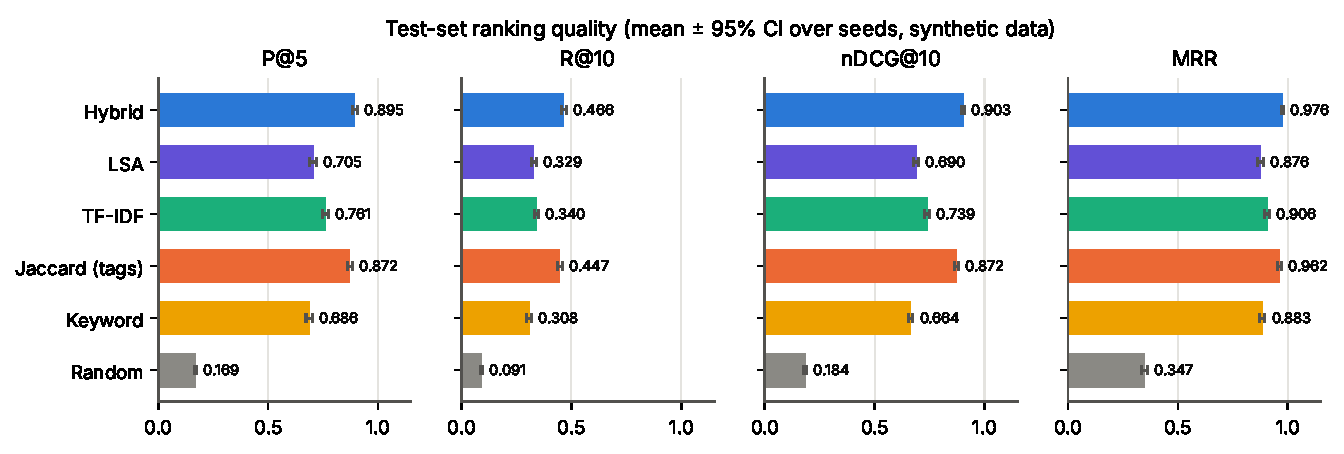
\includegraphics[width=\linewidth]{fig_main_metrics.pdf}
\caption{Test-set ranking quality of each method on real data (mean and 95\% CI over 20 random samples).}
\label{fig:main}
\end{figure}

Table~\ref{tab:sig} shows that the hybrid's advantage is consistent: it beat every baseline on nDCG@10 in all 20 samples, by $+0.114$ over tag matching (paired $t=29.6$), $+0.076$ over TF-IDF ($t=17.5$) and $+0.032$ over LSA ($t=12.1$); all $p$-values are below $10^{-4}$. On validation data, LSA was chosen as the text component in all 20 samples, with $\alpha=0.2$ in 17 samples and $\alpha=0.3$ in 3.

\begin{table}[htbp]
\centering
\small
\caption{Paired comparisons over the same 20 random samples (Hybrid minus baseline).}
\label{tab:sig}
\resizebox{\linewidth}{!}{%
\begin{tabular}{llrrrr}
\toprule
Baseline & Metric & Mean diff. & Paired $t$ ($p$) & Wilcoxon $p$ & Hybrid wins \\
\midrule
Jaccard (tags) & nDCG@10 & +0.114 & 29.6 (2.3e-17) & 1.9e-06 & 20/20 \\
Jaccard (tags) & P@5 & +0.113 & 21.6 (7.5e-15) & 8.8e-05 & 20/20 \\
TF-IDF & nDCG@10 & +0.076 & 17.5 (3.7e-13) & 1.9e-06 & 20/20 \\
TF-IDF & P@5 & +0.075 & 15.4 (3.5e-12) & 8.8e-05 & 20/20 \\
LSA & nDCG@10 & +0.032 & 12.1 (2.2e-10) & 1.9e-06 & 20/20 \\
LSA & P@5 & +0.042 & 10.9 (1.2e-09) & 8.8e-05 & 20/20 \\
\bottomrule
\end{tabular}}
\end{table}

Figure~\ref{fig:grid} shows the validation curve for sample 0. With LSA text, nDCG@10 rises from 0.342 (tags only, $\alpha=0$) to a peak of 0.450 at $\alpha=0.2$ and then slowly falls to 0.415 for text only. With TF-IDF text the best weight is higher ($\alpha=0.5$, 0.437). In both cases a mixture beats either pure source.

\begin{figure}[htbp]
\centering
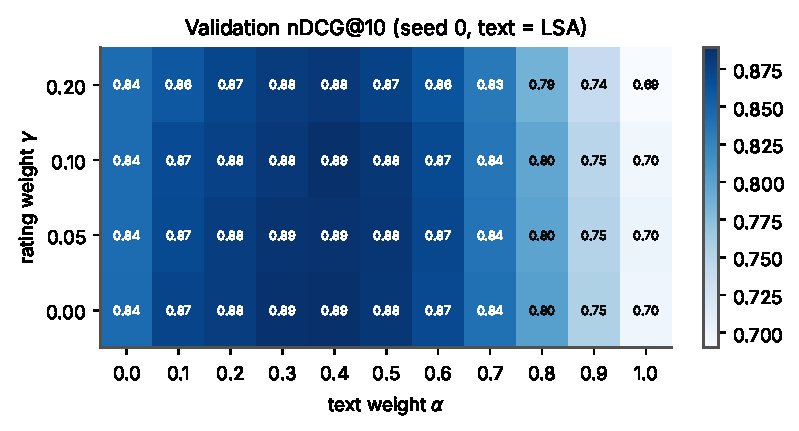
\includegraphics[width=0.62\linewidth]{fig_weight_grid.pdf}
\caption{Validation nDCG@10 as a function of the text weight $\alpha$ (sample 0).}
\label{fig:grid}
\end{figure}

\paragraph{Ablation.} Table~\ref{tab:ablation} changes one part of the tuned hybrid at a time. Replacing LSA by TF-IDF (re-tuned) lowers nDCG@10 from 0.438 to 0.412; text only gives 0.406, tags only 0.324, and a fixed equal weighting ($\alpha=0.5$) 0.420. Tuning $\alpha$ on validation data is therefore worth about 0.02 nDCG@10 over a reasonable default.

\begin{table}[htbp]
\centering
\small
\caption{Ablation of the hybrid model (test gigs, 20 samples, mean $\pm$ 95\% CI). $\alpha$ is the weight on text similarity; $1-\alpha$ goes to tag overlap.}
\label{tab:ablation}
\begin{tabular}{lcccc}
\toprule
Method & P@5 & R@100 & nDCG@10 & MRR \\
\midrule
Hybrid (tuned) & \textbf{0.389} $\pm$ 0.014 & 0.237 $\pm$ 0.006 & \textbf{0.438} $\pm$ 0.011 & \textbf{0.566} $\pm$ 0.014 \\
Hybrid, other text model & 0.363 $\pm$ 0.013 & 0.193 $\pm$ 0.004 & 0.412 $\pm$ 0.010 & 0.537 $\pm$ 0.016 \\
text only ($\alpha = 1$) & 0.348 $\pm$ 0.011 & 0.236 $\pm$ 0.006 & 0.406 $\pm$ 0.009 & 0.541 $\pm$ 0.012 \\
tags only ($\alpha = 0$) & 0.277 $\pm$ 0.012 & 0.124 $\pm$ 0.003 & 0.324 $\pm$ 0.010 & 0.462 $\pm$ 0.014 \\
equal weights ($\alpha = 0.5$) & 0.363 $\pm$ 0.012 & \textbf{0.240} $\pm$ 0.006 & 0.420 $\pm$ 0.010 & 0.551 $\pm$ 0.014 \\
\bottomrule
\end{tabular}
\end{table}

\paragraph{Differences between kinds of work.} Figure~\ref{fig:cat} breaks the test results down by Upwork category. The hybrid works well for visual and marketing work (\emph{Brand Identity Design} 0.85, \emph{SEO} 0.76, \emph{Logo Design} 0.76, \emph{Graphic Design} 0.75), and poorly for some technical and support work (\emph{Mobile App Development} 0.19, \emph{Data Analytics} 0.11, \emph{Email, Phone \& Chat Support} 0.07). It beat TF-IDF in most of the categories shown. Results per category are in \texttt{results/per\_category\_ndcg.csv}.

\begin{figure}[htbp]
\centering
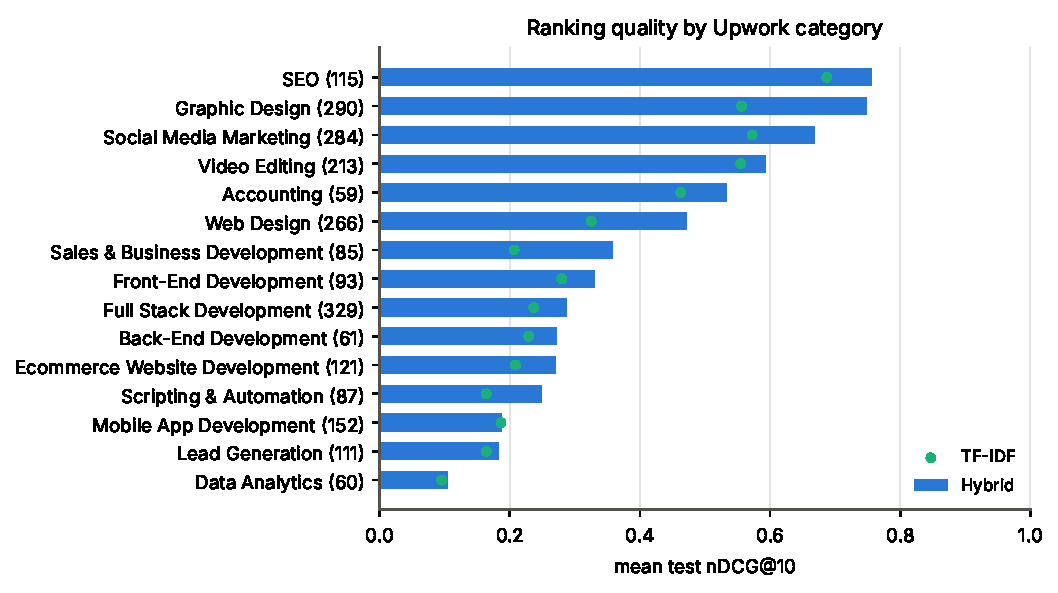
\includegraphics[width=0.78\linewidth]{fig_per_category.pdf}
\caption{Mean test nDCG@10 for the 15 most frequent Upwork categories (number of test gigs over all samples in brackets).}
\label{fig:cat}
\end{figure}

\subsection{Robustness to shorter profiles and missing tags (RQ2)}
Real seekers write profiles of very different length and list different numbers of skills. Figure~\ref{fig:robust} changes one of these at a time (5 samples per level, all 400 gigs, hybrid fixed at LSA with $\alpha=0.2$). When each resume is cut to its first 100 words, the hybrid keeps almost all of its accuracy (0.440 versus 0.452 for full resumes), while TF-IDF drops from 0.374 to 0.314; with only 25 words the hybrid still reaches 0.366, against 0.288 for LSA and 0.245 for TF-IDF. (Resume tags were taken from the full resume in this test, so tag matching does not change.) When seeker tags are deleted at random, tag matching falls from 0.323 to 0.224 at a deletion probability of 0.8. The hybrid degrades more slowly (0.452 to 0.375) but, with its weight fixed, it drops below LSA alone (0.420) once more than about half of the tags are missing.

\begin{figure}[htbp]
\centering
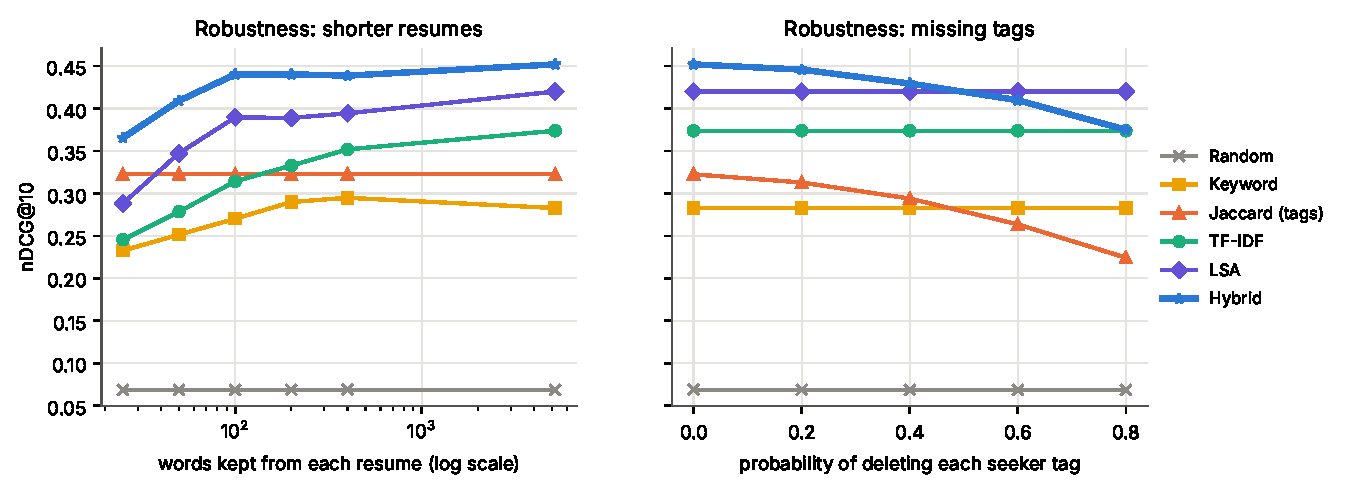
\includegraphics[width=\linewidth]{fig_robustness.pdf}
\caption{nDCG@10 when resumes are shortened (left) and when seeker tags are deleted at random (right); mean over 5 samples per level.}
\label{fig:robust}
\end{figure}

\subsection{Simultaneous assignment (RQ3)}
Table~\ref{tab:assign} matches all 400 sampled gigs at once using the tuned hybrid scores, both with all \DataSeekers{} resumes (surplus) and with a random 300 of them (scarce). Exact assignment never double-books and collects more relevance than greedy assignment: 325.8 versus 322.9 (+0.9\%) in the surplus market and 129.7 versus 122.2 (+6.1\%) in the scarce market. Letting each gig take its own best seeker (\enquote{independent top-1}) looks best on paper, but it gives the same resumes to many gigs at once (245.7 double bookings with all resumes and 309.6 with 300), which is not a valid plan. The exact solver was also much faster than our greedy loop (0.03~s versus 1.4~s for 400 gigs and \DataSeekers{} resumes).

\begin{table}[htbp]
\centering
\small
\caption{Simultaneous assignment of all 400 sampled gigs (mean over 20 samples). \emph{True relevance} sums the category-based relevance of the chosen pairs; \emph{good match rate} is the share of the gigs that receive a resume from the primary matching category ($\mathrm{rel}=2$).}
\label{tab:assign}
\resizebox{\linewidth}{!}{%
\begin{tabular}{llrrrrr}
\toprule
Market & Policy & Pred.\ utility & True relevance & Good match rate & Gigs filled & Double-booked \\
\midrule
surplus (2483 seekers) & Optimal (Hungarian) & 60.13 & 325.80 & 0.304 & 400.0 & 0.0 \\
 & Greedy & 58.58 & 322.85 & 0.303 & 400.0 & 0.0 \\
 & Independent top-1 & 68.85 & 414.45 & 0.437 & 400.0 & 245.7 \\
\midrule
scarce (300 seekers) & Optimal (Hungarian) & 33.60 & 129.65 & 0.115 & 300.0 & 0.0 \\
 & Greedy & 31.96 & 122.15 & 0.107 & 300.0 & 0.0 \\
 & Independent top-1 & 55.25 & 364.40 & 0.367 & 400.0 & 309.6 \\
\bottomrule
\end{tabular}}
\end{table}

\subsection{Numerical behaviour and cost (RQ4)}\label{sec:svdconv}
\paragraph{LSA rank.} Figure~\ref{fig:lsa} shows that LSA works best with a small number of concepts: nDCG@10 is 0.403 at $k=10$, peaks at 0.446 at $k=20$, is 0.420 at $k=40$ (our setting, chosen before the sweep), and falls to 0.367 at $k=320$, slightly below full-rank TF-IDF (0.374). A small $k$ keeps the broad \enquote{field of work} of a document and drops the many specific words in which job posts and resumes differ.

\paragraph{Randomized SVD convergence.} Table~\ref{tab:svd} and Figure~\ref{fig:svd} compare the singular values from the randomized solver with exact ARPACK values for the $2883\times41{,}587$ TF-IDF matrix of sample 0 ($k=40$). The error decreases steadily with the number of power iterations $q$: with $q=0$ the mean relative error is 44\%; with the setting used in this study, $q=7$, it is $2.0\times10^{-3}$ (largest $1.7\times10^{-2}$), and a mean error below $10^{-3}$ is first reached at $q=9$. The 40 components explain only 12.5\% of the variance, and the exact rank-40 approximation has relative Frobenius error $0.906$: LSA keeps a very small, coarse part of the word-level information, which is still enough to identify the field of work.

\begin{figure}[htbp]
\centering
\begin{subfigure}{0.49\linewidth}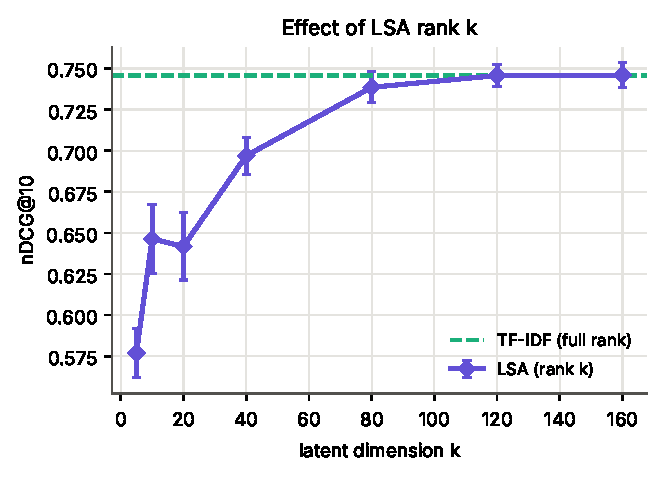
\includegraphics[width=\linewidth]{fig_lsa_rank.pdf}\caption{Effect of the LSA rank $k$ (5 samples, all gigs).}\label{fig:lsa}\end{subfigure}\hfill
\begin{subfigure}{0.49\linewidth}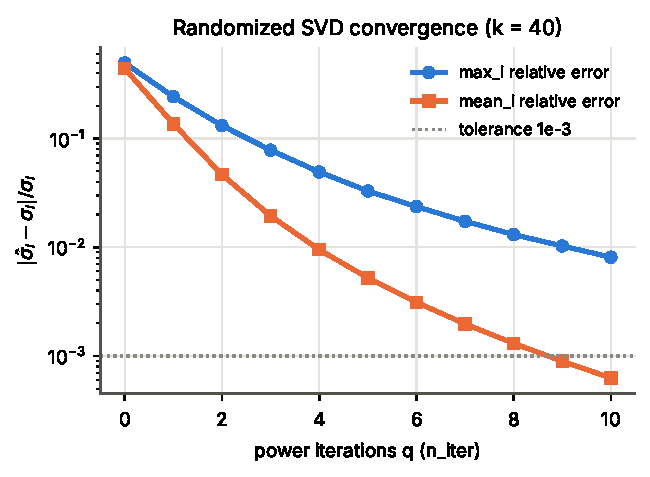
\includegraphics[width=\linewidth]{fig_svd_convergence.pdf}\caption{Relative singular-value error versus $q$.}\label{fig:svd}\end{subfigure}
\caption{Numerical behaviour of latent semantic analysis.}
\end{figure}

\begin{table}[htbp]
\centering
\small
\caption{Randomized SVD versus exact ARPACK singular values ($k=40$, matrix 2883$\times$41587, mean of 5 random starts).}
\label{tab:svd}
\begin{tabular}{rccc}
\toprule
$q$ & max rel.\ error & mean rel.\ error & explained variance \\
\midrule
0 & 4.97e-01 & 4.42e-01 & 0.0437 \\
1 & 2.43e-01 & 1.37e-01 & 0.1060 \\
2 & 1.32e-01 & 4.67e-02 & 0.1191 \\
4 & 4.93e-02 & 9.51e-03 & 0.1239 \\
6 & 2.36e-02 & 3.12e-03 & 0.1246 \\
7 & 1.74e-02 & 1.97e-03 & 0.1248 \\
8 & 1.31e-02 & 1.31e-03 & 0.1249 \\
10 & 8.10e-03 & 6.27e-04 & 0.1249 \\
\bottomrule
\end{tabular}
\end{table}

\paragraph{Monte Carlo convergence.} Figure~\ref{fig:mc} plots the running mean of test nDCG@10 as samples are added. The estimates stabilise after about 10 samples; at 20 samples the 95\% confidence half-width is 0.011 for the hybrid model, smaller than the gaps between methods.

\paragraph{Runtime.} Table~\ref{tab:runtime} and Figure~\ref{fig:runtime} report wall-clock times for $n$ gigs and $n$ resumes. For a campus-scale case ($n=400$), TF-IDF scoring takes about 0.5~s and exact assignment under 0.01~s. The fitted log--log slopes for $n\ge400$ are about 1.1 for TF-IDF scoring (sparse operations), 2.3 for the dense Jaccard matrix, 2.6 for exact assignment (below its $O(n^3)$ worst case) and 2.1 for the greedy method. Our greedy loop is plain Python while SciPy's solver is compiled code, which is why the exact solver was faster in practice. The complete set of experiments took about \DataRuntimeMin{} minutes.

\begin{figure}[htbp]
\centering
\begin{subfigure}{0.49\linewidth}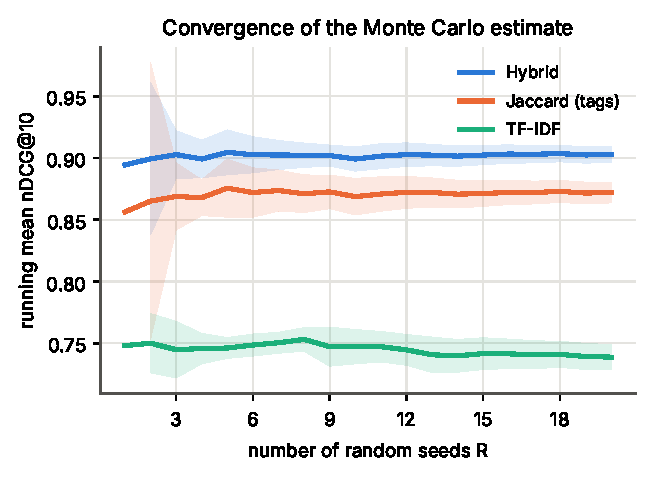
\includegraphics[width=\linewidth]{fig_monte_carlo.pdf}\caption{Running mean and 95\% CI over samples.}\label{fig:mc}\end{subfigure}\hfill
\begin{subfigure}{0.49\linewidth}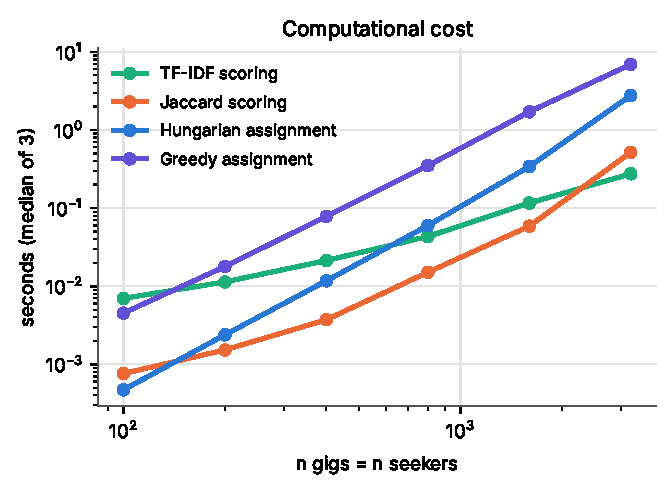
\includegraphics[width=\linewidth]{fig_runtime_scaling.pdf}\caption{Runtime versus problem size (log--log).}\label{fig:runtime}\end{subfigure}
\caption{Statistical convergence of the estimates and computational cost.}
\end{figure}

\begin{table}[htbp]
\centering
\small
\caption{Wall-clock time in seconds (median of 3 runs) for $n$ gigs and $n$ seekers. The last row is the slope of a least-squares line fitted to $\log t$ versus $\log n$ for $n \ge 400$ (empirical complexity exponent).}
\label{tab:runtime}
\begin{tabular}{rrrrr}
\toprule
$n$ & TF-IDF scoring & Jaccard scoring & Hungarian & Greedy \\
\midrule
100 & 0.1244 & 0.0034 & 0.0004 & 0.0104 \\
200 & 0.2753 & 0.0070 & 0.0018 & 0.0418 \\
400 & 0.4859 & 0.0161 & 0.0084 & 0.1873 \\
800 & 0.9879 & 0.0584 & 0.0408 & 0.7631 \\
1600 & 2.0359 & 0.3454 & 0.2600 & 3.4574 \\
2400 & 3.4450 & 0.8729 & 0.8297 & 8.3417 \\
\midrule
slope & 1.08 & 2.26 & 2.57 & 2.12 \\
\bottomrule
\end{tabular}
\end{table}

% ---------------------------------------------------------------------
\section{Analysis and Discussion}\label{sec:discussion}

\paragraph{Accuracy.} On real data the task is much harder than on a clean, generated dataset: job posts are short and specific, resumes are long and cover a whole career, and the two are written by different people for different purposes. Even so, every content-based method was four to six times better than random ranking, and the hybrid placed a right-field resume first for most gigs (MRR 0.566). An absolute nDCG@10 of 0.44 should be read together with the strict ground truth: a resume counts as fully relevant only when its LiveCareer category is the primary match, so a web designer filed under \textsc{arts} gets only partial credit for a \emph{Web Design} gig.

\paragraph{Why the hybrid helps.} Tags and text fail in different ways. The Upwork tags of a gig are precise, but a resume's tags come from exact phrase matches and include many generic words (\emph{business}, \emph{development}), so tag overlap alone is noisy. Free text carries the field of work but also much unrelated detail. Combining them (Eq.~\ref{eq:hybrid}) was more accurate than either alone in every sample. The selected $\alpha=0.2$ puts a weight of 0.8 on tags in the formula, but this does not mean that tags dominate: Jaccard values between a short tag list and a long resume are small (99\% of pairs below 0.07, standard deviation 0.013), while LSA cosines spread much more (standard deviation 0.12). After weighting, the text term still varies about twice as much as the tag term, and the tags mainly lift resumes that share the gig's exact skills.

\paragraph{The role of LSA.} On real data LSA clearly beat TF-IDF (0.406 versus 0.362), and it did best with only about 20--40 concepts. Real job posts and resumes rarely use the same exact words for the same work, and a low-rank concept space groups words that tend to occur together in one field (for example \emph{photoshop}, \emph{illustrator}, \emph{branding}). This is the vocabulary-mismatch benefit that motivated LSA (Section~\ref{sec:prelim}).

\paragraph{Where it fails.} The weakest categories are those whose words are shared by many fields or whose workers are spread over several resume categories. \emph{Data Analytics} posts resemble resumes in finance, IT, engineering and consulting; \emph{Email, Phone \& Chat Support} posts resemble any customer-facing resume; and software posts are split between \textsc{information-technology} and \textsc{engineering} resumes. Part of this error comes from the coarse 24-category ground truth rather than from the model.

\paragraph{Stability.} Results varied little across samples (standard deviation of the hybrid's nDCG@10 is 0.023), the chosen weights were very stable (LSA with $\alpha\in\{0.2,0.3\}$ in all samples), and the validation curve is flat near its optimum (Figure~\ref{fig:grid}). Numerically, the randomized SVD converges reliably; at $q=7$ the singular values are accurate to about two to three significant figures, which does not change the rankings in a meaningful way, and $q=9$ would meet a $10^{-3}$ tolerance.

\paragraph{Computational cost.} At GigLink's expected scale (hundreds of gigs and seekers) all steps take about a second or less on a laptop, so matching can be recomputed whenever a gig is posted. Exact assignment grows roughly like $n^{2.6}$ in our tests; for thousands of simultaneous gigs the problem could be split by category or restricted to each gig's top candidates.

\paragraph{Practical significance for GigLink.} The method can power two features: (i) a ranked \enquote{suggested seekers} list on each gig page, with an explanation of which tags and words matched; and (ii) a batch matching step that spreads opportunities across seekers instead of sending every client to the same few people. The per-category results suggest that GigLink can rely on the matcher first for design, media and marketing gigs, which are also common student gigs, and should treat suggestions for technical and support gigs with more care.

\subsection{Limitations and sources of error}\label{sec:limits}
\begin{itemize}[nosep]
  \item \textbf{Proxy data.} The gigs are Upwork posts and the seekers are LiveCareer resumes, not GigLink users. Student profiles will be shorter, and real GigLink posts may be in Filipino or Taglish; the absolute values may differ on GigLink data.
  \item \textbf{Ground-truth definition.} Relevance is judged by job category through a table that we wrote by hand (\texttt{data/category\_map.csv}). It is coarse (24 resume categories), it reflects our judgement, and it ignores quality, price and availability (Assumption~\ref{as:gt}). A different table would give different numbers. Real hiring outcomes would be a better ground truth.
  \item \textbf{Constraints not tested.} The resumes contain no schedule, hourly rate or rating, so the feasibility filter (Eq.~\ref{eq:feas}) and a reputation term could not be evaluated.
  \item \textbf{Generated tags for seekers.} Resume tags come from exact phrase matching against Upwork tags, which misses synonyms and adds generic words.
  \item \textbf{Static, one-to-one matching.} Real seekers can take several small gigs, and gigs arrive over time. Capacities and online matching are not modelled.
  \item \textbf{Fairness.} Ranking can concentrate opportunities on a few profiles. We did not audit fairness.
  \item \textbf{Hyperparameter selection} used a single random validation split per sample, and the LSA rank $k=40$ was fixed before the rank sweep, which later showed $k=20$ to be slightly better.
\end{itemize}

\begin{table}[htbp]
\centering\small
\caption{Status of each component of this study.}\label{tab:status}
\begin{tabular}{>{\raggedright\arraybackslash}p{0.52\linewidth}>{\raggedright\arraybackslash}p{0.4\linewidth}}
\toprule
Component & Status \\
\midrule
Real-data loader, category table, TF-IDF/LSA/Jaccard/hybrid models, metrics, assignment & Implemented and unit-tested (9 tests) \\
Offline evaluation on real Upwork posts and resumes, robustness, convergence and runtime experiments & Run; results reported here \\
Command-line demo and Google Colab notebook & Implemented; use the real resumes \\
Schedule and budget constraints & Implemented in code; \textbf{not evaluated} (no data) \\
Integration into the GigLink web application (API endpoint, UI) & \textbf{Proposed}, not implemented \\
Evaluation on GigLink postings and hiring outcomes & \textbf{Requires data}; not done \\
User study, fairness audit, online A/B test & \textbf{Proposed}; not done \\
\bottomrule
\end{tabular}
\end{table}

% ---------------------------------------------------------------------
\section{Conclusion}\label{sec:conclusion}
We formulated GigLink's provider-matching module as content-based ranking followed by a linear assignment problem, and implemented it with TF-IDF, latent semantic analysis computed by randomized SVD, Jaccard tag similarity and the Hungarian-type exact assignment solver. On real public data, 42,029 Upwork job posts matched against 2,483 real resumes, the hybrid model reached a test nDCG@10 of 0.438 and a P@5 of 0.389, consistently above LSA (0.406), TF-IDF (0.362), tag matching (0.324) and random ranking (0.068) in all 20 samples. LSA was the most useful text representation on real text, the hybrid stayed accurate even when resumes were cut to 100 words, and accuracy was high for design and marketing gigs but low for data-analytics and support gigs. Exact assignment produced conflict-free simultaneous matches with more total relevance than a greedy heuristic, especially when seekers were scarce, and the whole pipeline runs in about a second at campus scale.

These results suggest that a simple, explainable linear-algebra model is a feasible first AI component for GigLink, and that it can be demonstrated today with the accompanying command-line program and Colab notebook.

% ---------------------------------------------------------------------
\section{Recommendations and Future Directions}\label{sec:future}
\begin{enumerate}[label=\arabic*.]
  \item \textbf{Validate on GigLink data.} Collect anonymised, consented GigLink postings, profiles and hiring outcomes, re-tune $\alpha$ and $k$ on them, and replace the category table with real outcomes as ground truth.
  \item \textbf{Evaluate the constraints.} Once seekers state their availability and rates, measure the effect of the schedule and budget filter (Eq.~\ref{eq:feas}).
  \item \textbf{Filipino and Taglish text.} Complement TF-IDF/LSA with multilingual sentence embeddings and compare them under the same evaluation protocol.
  \item \textbf{Better seeker tags.} Let seekers choose tags from the same list as clients, or learn synonyms, instead of exact phrase matching.
  \item \textbf{Richer assignment.} Allow seekers to take several small gigs (capacity constraints) and match gigs as they arrive over time (online assignment).
  \item \textbf{Fairness and integration.} Audit how often new seekers are recommended, and expose the matcher as an API endpoint in the GigLink web application with the explanation (matched tags and words) next to each suggestion.
\end{enumerate}

% ---------------------------------------------------------------------

\newpage

\begin{thebibliography}{99}
\addcontentsline{toc}{section}{References}

\bibitem[asaniczka(2024)]{upworkdata}
asaniczka. (2024). \textit{Upwork job postings dataset 2024 (50K records)} [Data set]. Kaggle. \url{https://www.kaggle.com/datasets/asaniczka/upwork-job-postings-dataset-2024-50k-records}

\bibitem[Bhawal(2021)]{resumedata}
Bhawal, S. (2021). \textit{Resume dataset} [Data set]. Kaggle. \url{https://www.kaggle.com/datasets/snehaanbhawal/resume-dataset}

\bibitem[Crouse(2016)]{crouse2016implementing}
Crouse, D.~F. (2016). On implementing 2D rectangular assignment algorithms. \textit{IEEE Transactions on Aerospace and Electronic Systems}, \textit{52}(4), 1679--1696. \url{https://doi.org/10.1109/TAES.2016.140952}

\bibitem[de~Ruijt \& Bhulai(2021)]{deruijt2021job}
de~Ruijt, C., \& Bhulai, S. (2021). \textit{Job recommender systems: A review} (arXiv:2111.13576). arXiv. \url{https://arxiv.org/abs/2111.13576}

\bibitem[Deerwester et~al.(1990)]{deerwester1990lsa}
Deerwester, S., Dumais, S.~T., Furnas, G.~W., Landauer, T.~K., \& Harshman, R. (1990). Indexing by latent semantic analysis. \textit{Journal of the American Society for Information Science}, \textit{41}(6), 391--407. \url{https://doi.org/10.1002/(SICI)1097-4571(199009)41:6<391::AID-ASI1>3.0.CO;2-9}

\bibitem[Eckart \& Young(1936)]{eckart1936approximation}
Eckart, C., \& Young, G. (1936). The approximation of one matrix by another of lower rank. \textit{Psychometrika}, \textit{1}(3), 211--218. \url{https://doi.org/10.1007/BF02288367}

\bibitem[Freire \& de~Castro(2021)]{freire2021erecruitment}
Freire, M.~N., \& de~Castro, L.~N. (2021). e-Recruitment recommender systems: A systematic review. \textit{Knowledge and Information Systems}, \textit{63}(1), 1--20. \url{https://doi.org/10.1007/s10115-020-01522-8}

\bibitem[Halko et~al.(2011)]{halko2011finding}
Halko, N., Martinsson, P.-G., \& Tropp, J.~A. (2011). Finding structure with randomness: Probabilistic algorithms for constructing approximate matrix decompositions. \textit{SIAM Review}, \textit{53}(2), 217--288. \url{https://doi.org/10.1137/090771806}

\bibitem[Harris et~al.(2020)]{harris2020numpy}
Harris, C.~R., Millman, K.~J., van~der Walt, S.~J., Gommers, R., Virtanen, P., Cournapeau, D., Wieser, E., Taylor, J., Berg, S., Smith, N.~J., Kern, R., Picus, M., Hoyer, S., van~Kerkwijk, M.~H., Brett, M., Haldane, A., del~R\'{i}o, J.~F., Wiebe, M., Peterson, P., \ldots{} Oliphant, T.~E. (2020). Array programming with NumPy. \textit{Nature}, \textit{585}(7825), 357--362. \url{https://doi.org/10.1038/s41586-020-2649-2}

\bibitem[Hunter(2007)]{hunter2007matplotlib}
Hunter, J.~D. (2007). Matplotlib: A 2D graphics environment. \textit{Computing in Science \& Engineering}, \textit{9}(3), 90--95. \url{https://doi.org/10.1109/MCSE.2007.55}

\bibitem[J\"{a}rvelin \& Kek\"{a}l\"{a}inen(2002)]{jarvelin2002cumulated}
J\"{a}rvelin, K., \& Kek\"{a}l\"{a}inen, J. (2002). Cumulated gain-based evaluation of IR techniques. \textit{ACM Transactions on Information Systems}, \textit{20}(4), 422--446. \url{https://doi.org/10.1145/582415.582418}

\bibitem[Kuhn(1955)]{kuhn1955hungarian}
Kuhn, H.~W. (1955). The Hungarian method for the assignment problem. \textit{Naval Research Logistics Quarterly}, \textit{2}(1--2), 83--97. \url{https://doi.org/10.1002/nav.3800020109}

\bibitem[Lops et~al.(2011)]{lops2011content}
Lops, P., de~Gemmis, M., \& Semeraro, G. (2011). Content-based recommender systems: State of the art and trends. In F.~Ricci, L.~Rokach, B.~Shapira, \& P.~B. Kantor (Eds.), \textit{Recommender systems handbook} (pp.~73--105). Springer. \url{https://doi.org/10.1007/978-0-387-85820-3_3}

\bibitem[Manning et~al.(2008)]{manning2008introduction}
Manning, C.~D., Raghavan, P., \& Sch\"{u}tze, H. (2008). \textit{Introduction to information retrieval}. Cambridge University Press.

\bibitem[Pedregosa et~al.(2011)]{pedregosa2011scikit}
Pedregosa, F., Varoquaux, G., Gramfort, A., Michel, V., Thirion, B., Grisel, O., Blondel, M., Prettenhofer, P., Weiss, R., Dubourg, V., Vanderplas, J., Passos, A., Cournapeau, D., Brucher, M., Perrot, M., \& Duchesnay, \'{E}. (2011). Scikit-learn: Machine learning in Python. \textit{Journal of Machine Learning Research}, \textit{12}, 2825--2830. \url{https://jmlr.org/papers/v12/pedregosa11a.html}

\bibitem[Ren et~al.(2023)]{ren2023hiring}
Ren, J., Raghupathi, V., \& Raghupathi, W. (2023). Exploring influential factors in hiring freelancers in online labor platforms: An empirical study. \textit{Economies}, \textit{11}(3), Article~80. \url{https://doi.org/10.3390/economies11030080}

\bibitem[Russell \& Norvig(2021)]{russell2021aima}
Russell, S.~J., \& Norvig, P. (2021). \textit{Artificial intelligence: A modern approach} (4th ed.). Pearson.

\bibitem[Salton \& Buckley(1988)]{salton1988term}
Salton, G., \& Buckley, C. (1988). Term-weighting approaches in automatic text retrieval. \textit{Information Processing \& Management}, \textit{24}(5), 513--523. \url{https://doi.org/10.1016/0306-4573(88)90021-0}

\bibitem[Salton et~al.(1975)]{salton1975vector}
Salton, G., Wong, A., \& Yang, C.-S. (1975). A vector space model for automatic indexing. \textit{Communications of the ACM}, \textit{18}(11), 613--620. \url{https://doi.org/10.1145/361219.361220}

\bibitem[Virtanen et~al.(2020)]{virtanen2020scipy}
Virtanen, P., Gommers, R., Oliphant, T.~E., Haberland, M., Reddy, T., Cournapeau, D., Burovski, E., Peterson, P., Weckesser, W., Bright, J., van~der Walt, S.~J., Brett, M., Wilson, J., Millman, K.~J., Mayorov, N., Nelson, A.~R.~J., Jones, E., Kern, R., Larson, E., \ldots{} SciPy 1.0 Contributors. (2020). SciPy 1.0: Fundamental algorithms for scientific computing in Python. \textit{Nature Methods}, \textit{17}(3), 261--272. \url{https://doi.org/10.1038/s41592-019-0686-2}

\bibitem[Wilcoxon(1945)]{wilcoxon1945individual}
Wilcoxon, F. (1945). Individual comparisons by ranking methods. \textit{Biometrics Bulletin}, \textit{1}(6), 80--83. \url{https://doi.org/10.2307/3001968}

\bibitem[Zhao et~al.(2021)]{zhao2021embedding}
Zhao, J., Wang, J., Sigdel, M., Zhang, B., Hoang, P., Liu, M., \& Korayem, M. (2021). \textit{Embedding-based recommender system for job to candidate matching on scale} (arXiv:2107.00221). arXiv. \url{https://arxiv.org/abs/2107.00221}

\end{thebibliography}

\newpage
\appendix
\section{Reproducing the Results}\label{app:repro}
All code, results and this paper's source are in the project's GitHub repository. The two raw Kaggle files are not stored in the repository; download them \citep{upworkdata,resumedata} into \texttt{data/raw/} first (see \texttt{data/raw/README.md}). From the repository root:
\begin{lstlisting}[language=bash,numbers=none]
python -m venv .venv && source .venv/bin/activate   # Windows: .venv\Scripts\activate
pip install -r requirements.txt
python -m pytest -q                  # 9 unit tests
python -m giglink_ai.experiments     # all experiments, figures and tables
python -m giglink_ai.demo            # try the matcher on a sample gig
cd paper && latexmk -pdf main.tex    # rebuild this paper
\end{lstlisting}
Because every random draw is seeded, the metric values are identical on every run; only the runtime measurements depend on the machine. The notebook \texttt{notebooks/GigLink\_Colab.ipynb} runs the same code in Google Colab.

\section{Ranking Metrics Code}\label{app:metrics}
\begin{lstlisting}[caption={Precision@$k$ and nDCG@$k$ (excerpt of \texttt{giglink\_ai/metrics.py}).}]
def _topk(scores, k):
    order = np.argsort(-scores, axis=1, kind="stable")
    return order[:, :k]

def precision_at_k(scores, rel, k=5, threshold=2):
    top = _topk(scores, k)
    hits = np.take_along_axis(rel, top, axis=1) >= threshold
    return float(hits.mean())

def ndcg_at_k(scores, rel, k=10):
    discounts = 1.0 / np.log2(np.arange(2, k + 2))
    top = _topk(scores, k)
    gains = 2.0 ** np.take_along_axis(rel, top, axis=1) - 1
    dcg = (gains * discounts).sum(axis=1)
    ideal = 2.0 ** (-np.sort(-rel, axis=1)[:, :k]) - 1
    idcg = (ideal * discounts).sum(axis=1)
    mask = idcg > 0
    return float((dcg[mask] / idcg[mask]).mean())
\end{lstlisting}

\end{document}
